\section{User Interface Prototype}

\begin{figure}[!h]
    \begin{minipage}{0.3\textwidth}
        \centering
        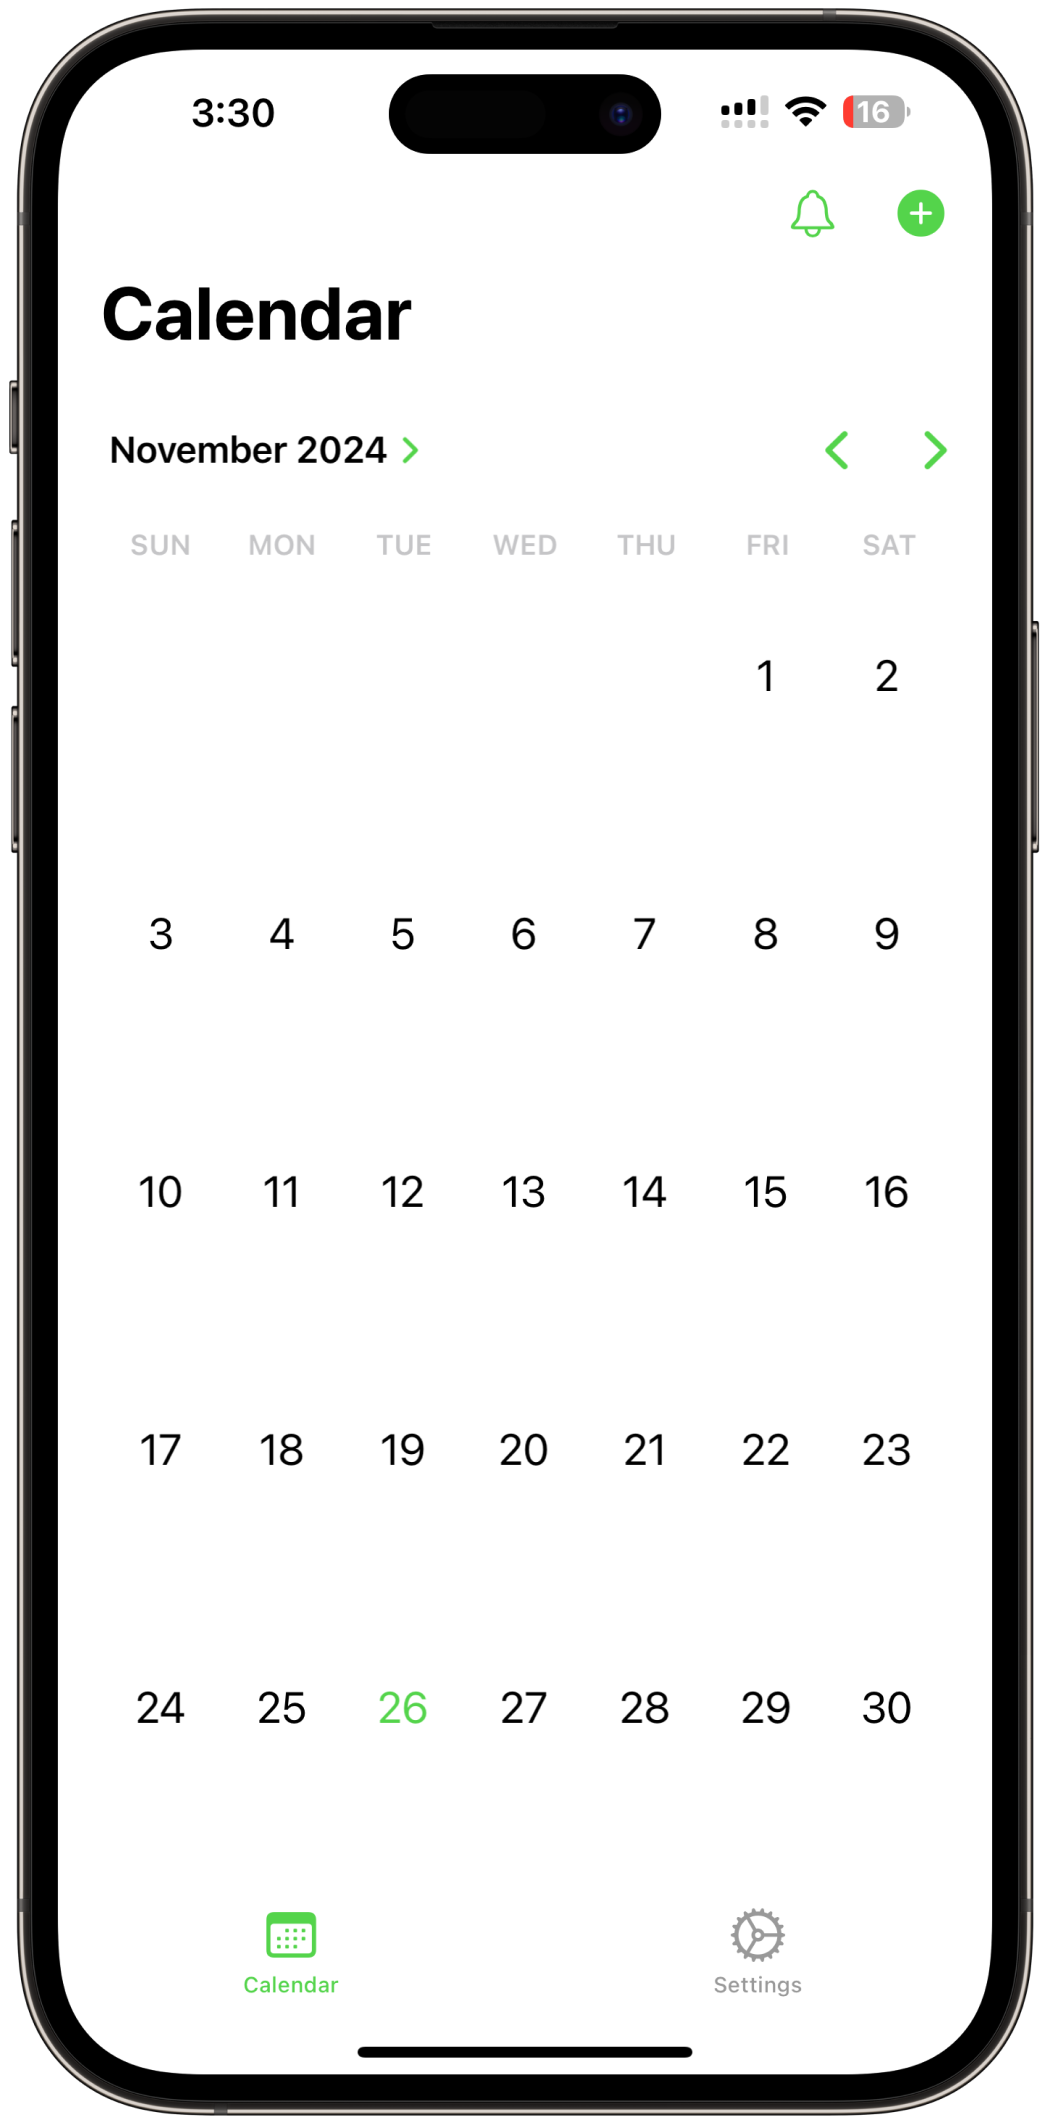
\includegraphics[width=\textwidth]{images/screen1.png}
        \caption{UI Screen 1: Calendar View}
        \label{fig:ui-screen-1}
    \end{minipage}
    \hfill
    \begin{minipage}{0.65\textwidth}
        In Figure \ref{fig:ui-screen-1}, the calendar view represents the user's schedule. It shows upcoming events, past events, and current events. It also has two buttons at the top, notifications and add event buttons. Users can swipe left and right to navigate months. The current day is colored in green.
    \end{minipage}
\end{figure}

\begin{figure}[!h]
    \begin{minipage}{0.65\textwidth}
        In Figure \ref{fig:ui-screen-2}, users can click on the text that shows the currently selected month, in this case ``November 2024'' and get a selector wheel that allows them to choose a month and a year to navigate to.
    \end{minipage}
    \hfill
    \begin{minipage}{0.3\textwidth}
        \centering
        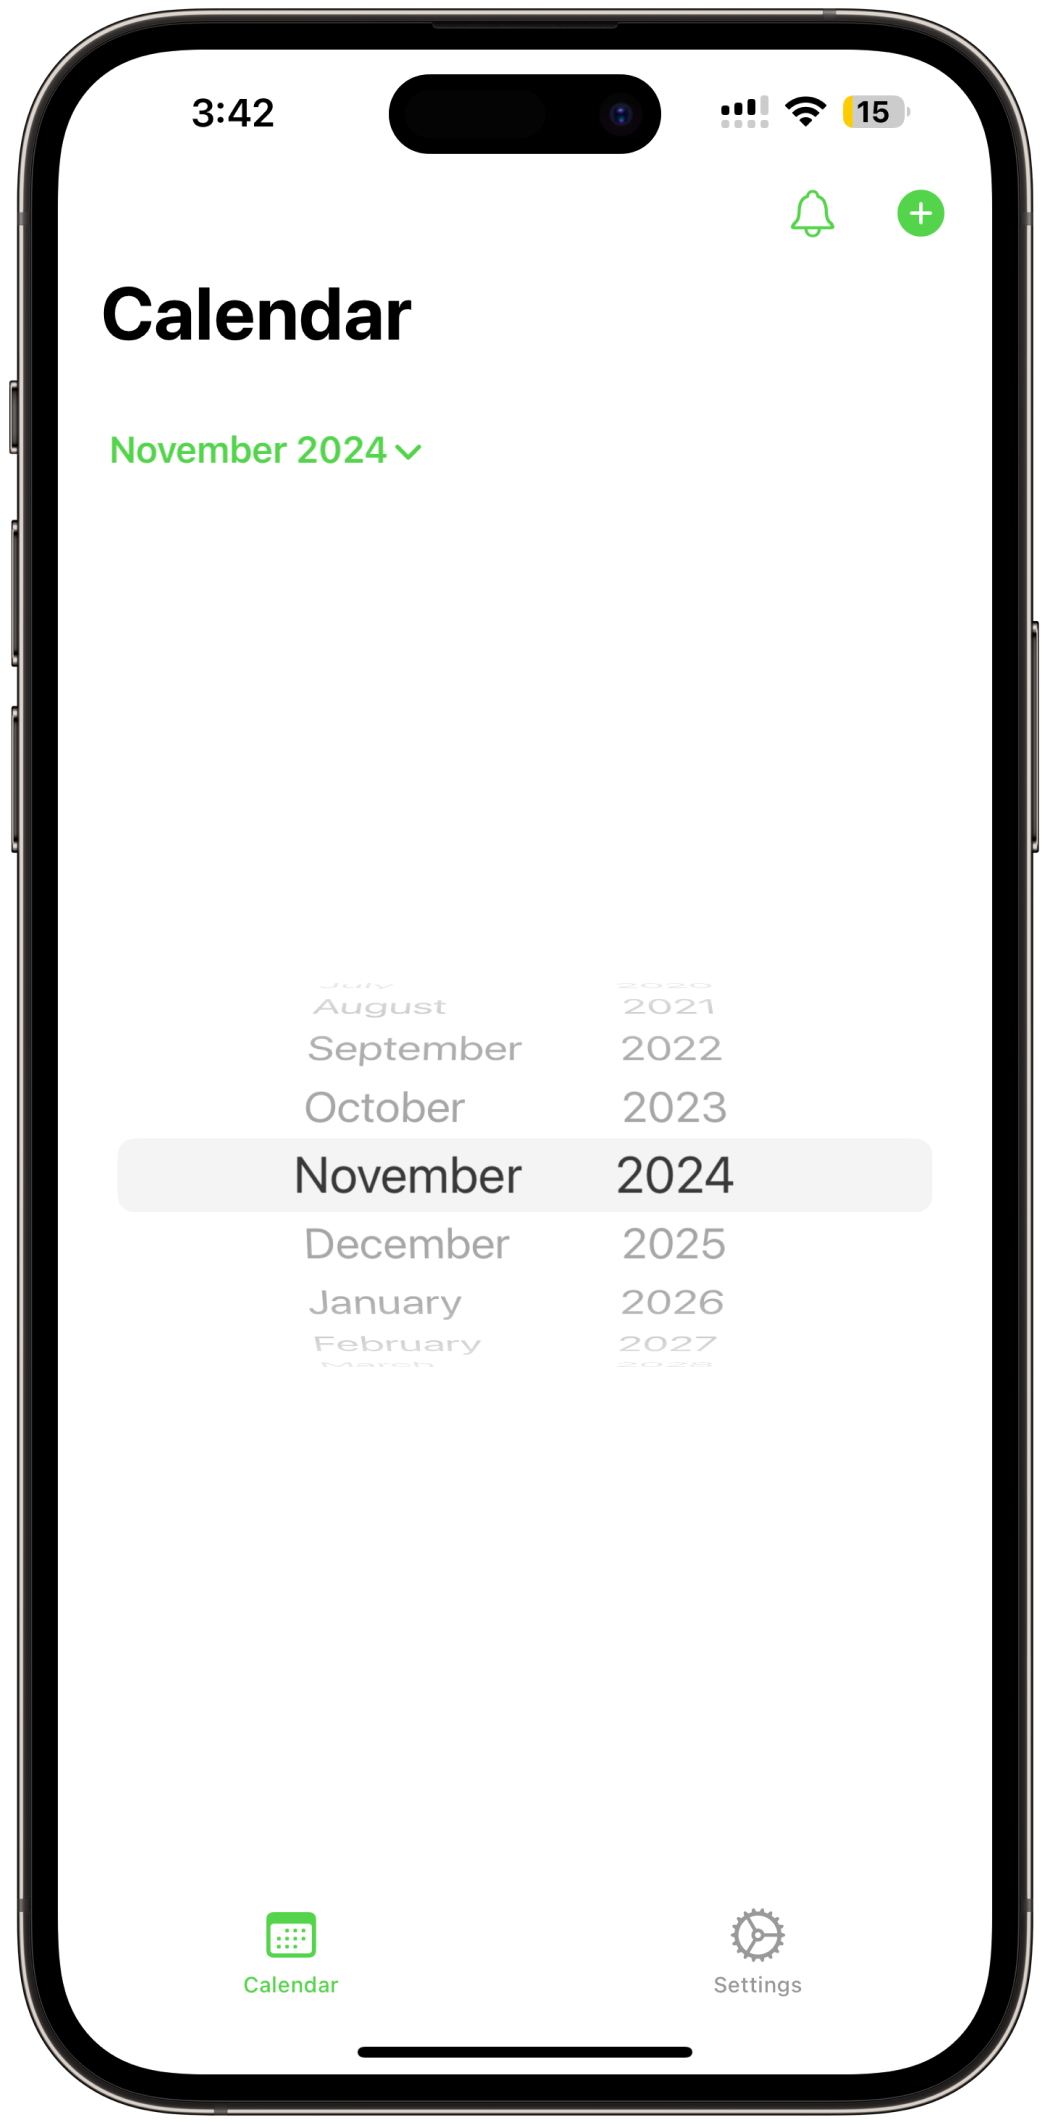
\includegraphics[width=\textwidth]{images/screen2.png}
        \caption{UI Screen 2: Month \& Year Selector}
        \label{fig:ui-screen-2}
    \end{minipage}
\end{figure}

\begin{figure}[!h]
    \begin{minipage}{0.3\textwidth}
        \centering
        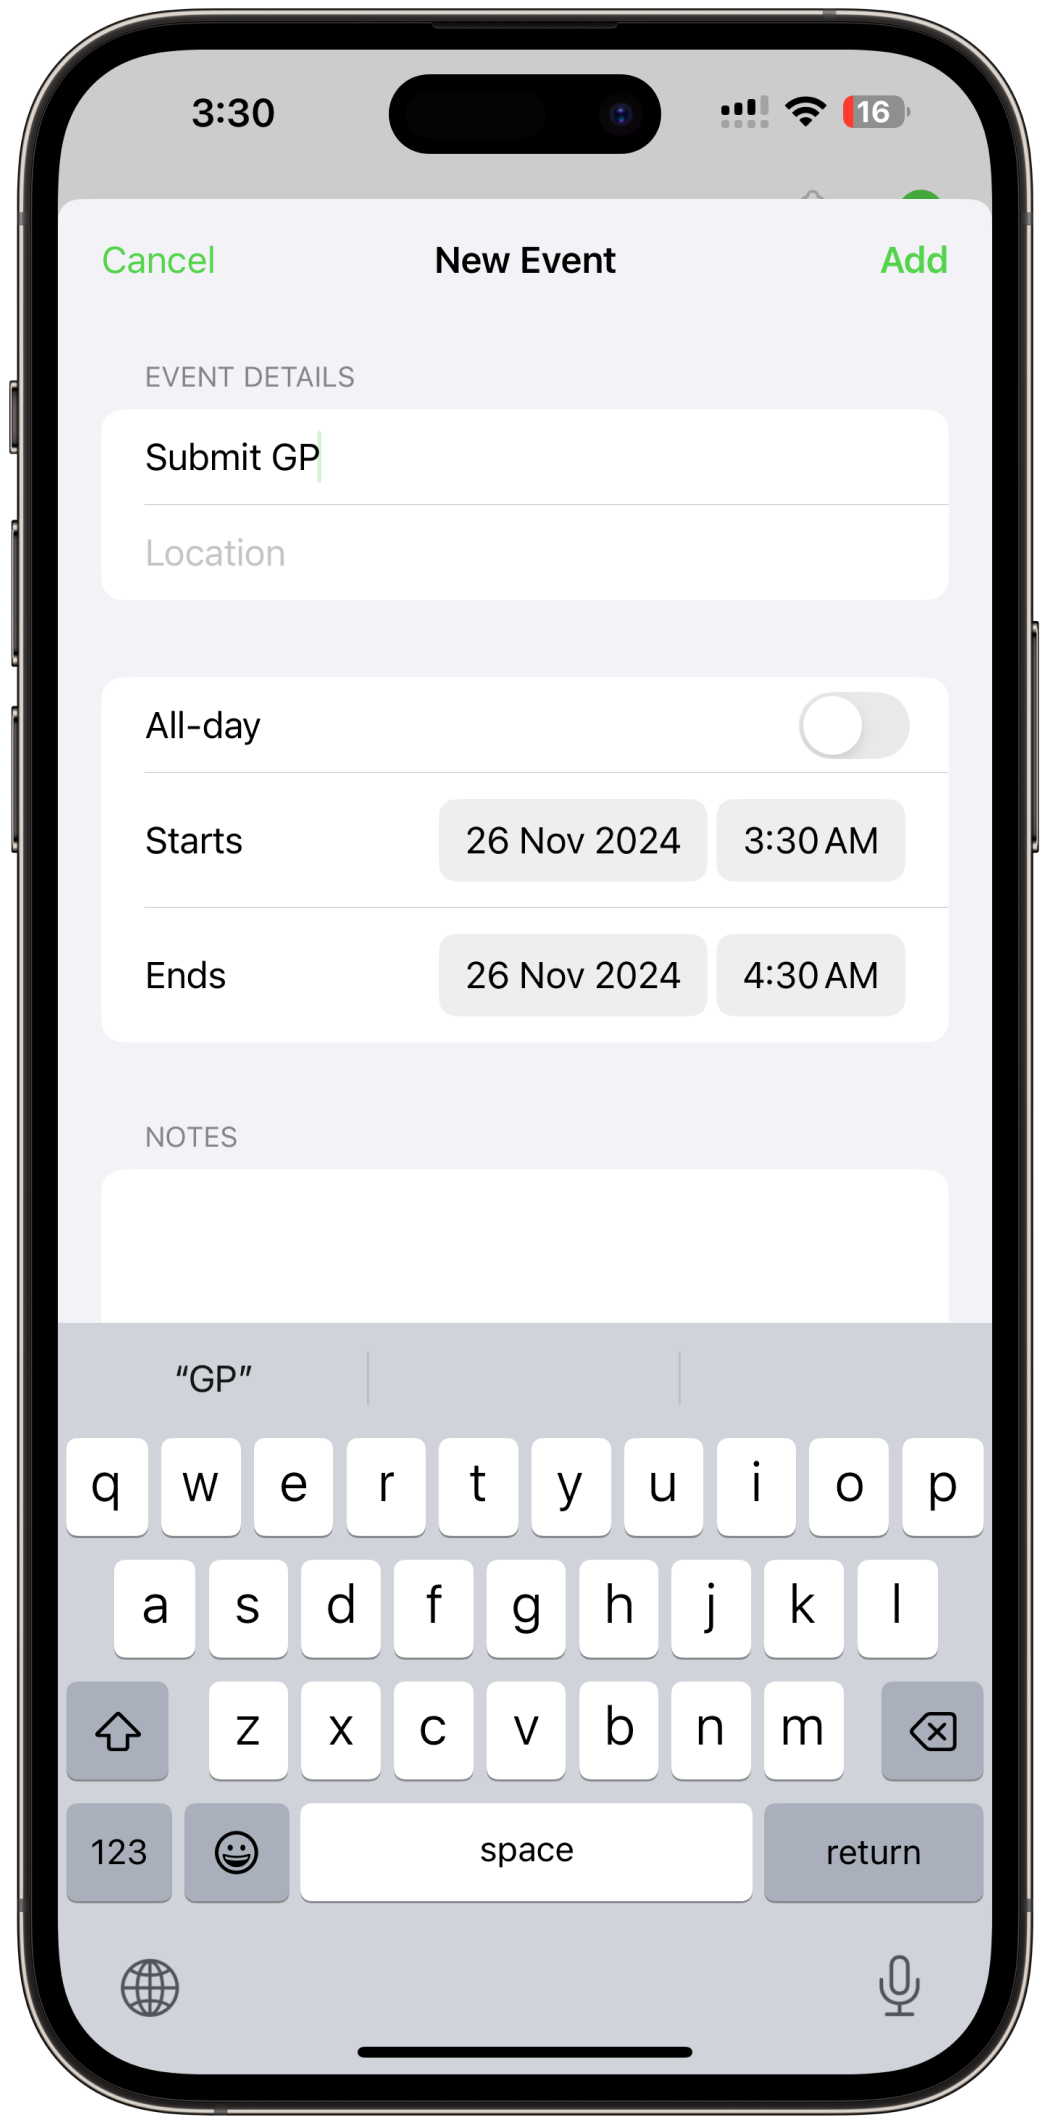
\includegraphics[width=\textwidth]{images/screen3.png}
        \caption{UI Screen 3: Add Event View - Default}
        \label{fig:ui-screen-3}
    \end{minipage}
    \hfill
    \begin{minipage}{0.65\textwidth}
        Your explanation for Screen 3 goes here. This text will appear to the right 
        of the third screenshot. You can describe the final state of the interface 
        and what the user can accomplish on this screen.
    \end{minipage}
\end{figure}

\begin{figure}[!h]
    \begin{minipage}{0.65\textwidth}
        Your explanation for Screen 3 goes here. This text will appear to the right 
        of the third screenshot. You can describe the final state of the interface 
        and what the user can accomplish on this screen.
    \end{minipage}
    \hfill
    \begin{minipage}{0.3\textwidth}
        \centering
        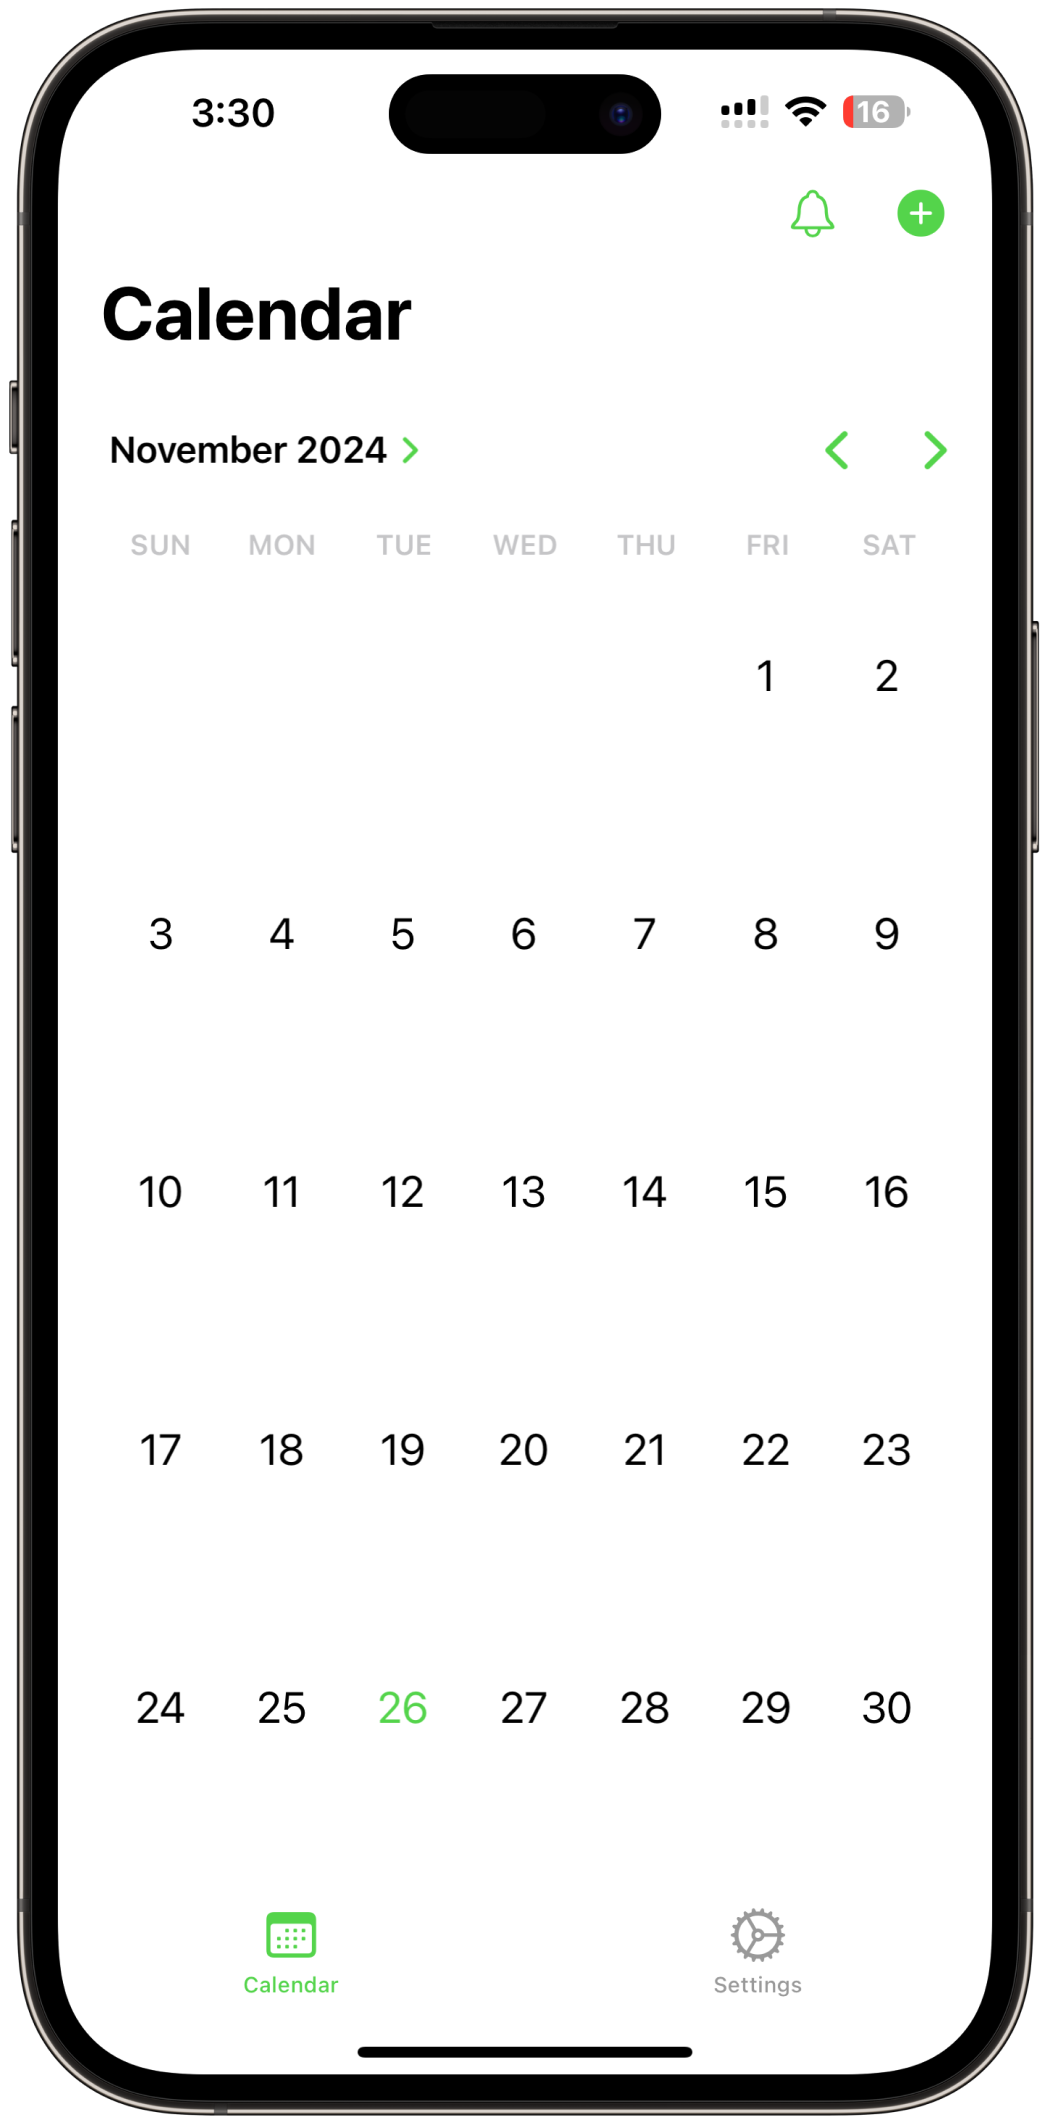
\includegraphics[width=\textwidth]{images/screen4.png}
        \caption{UI Screen 4: Add Event View - Date Selector}
        \label{fig:ui-screen-4}
    \end{minipage}
\end{figure}

\begin{figure}[!h]
    \begin{minipage}{0.3\textwidth}
        \centering
        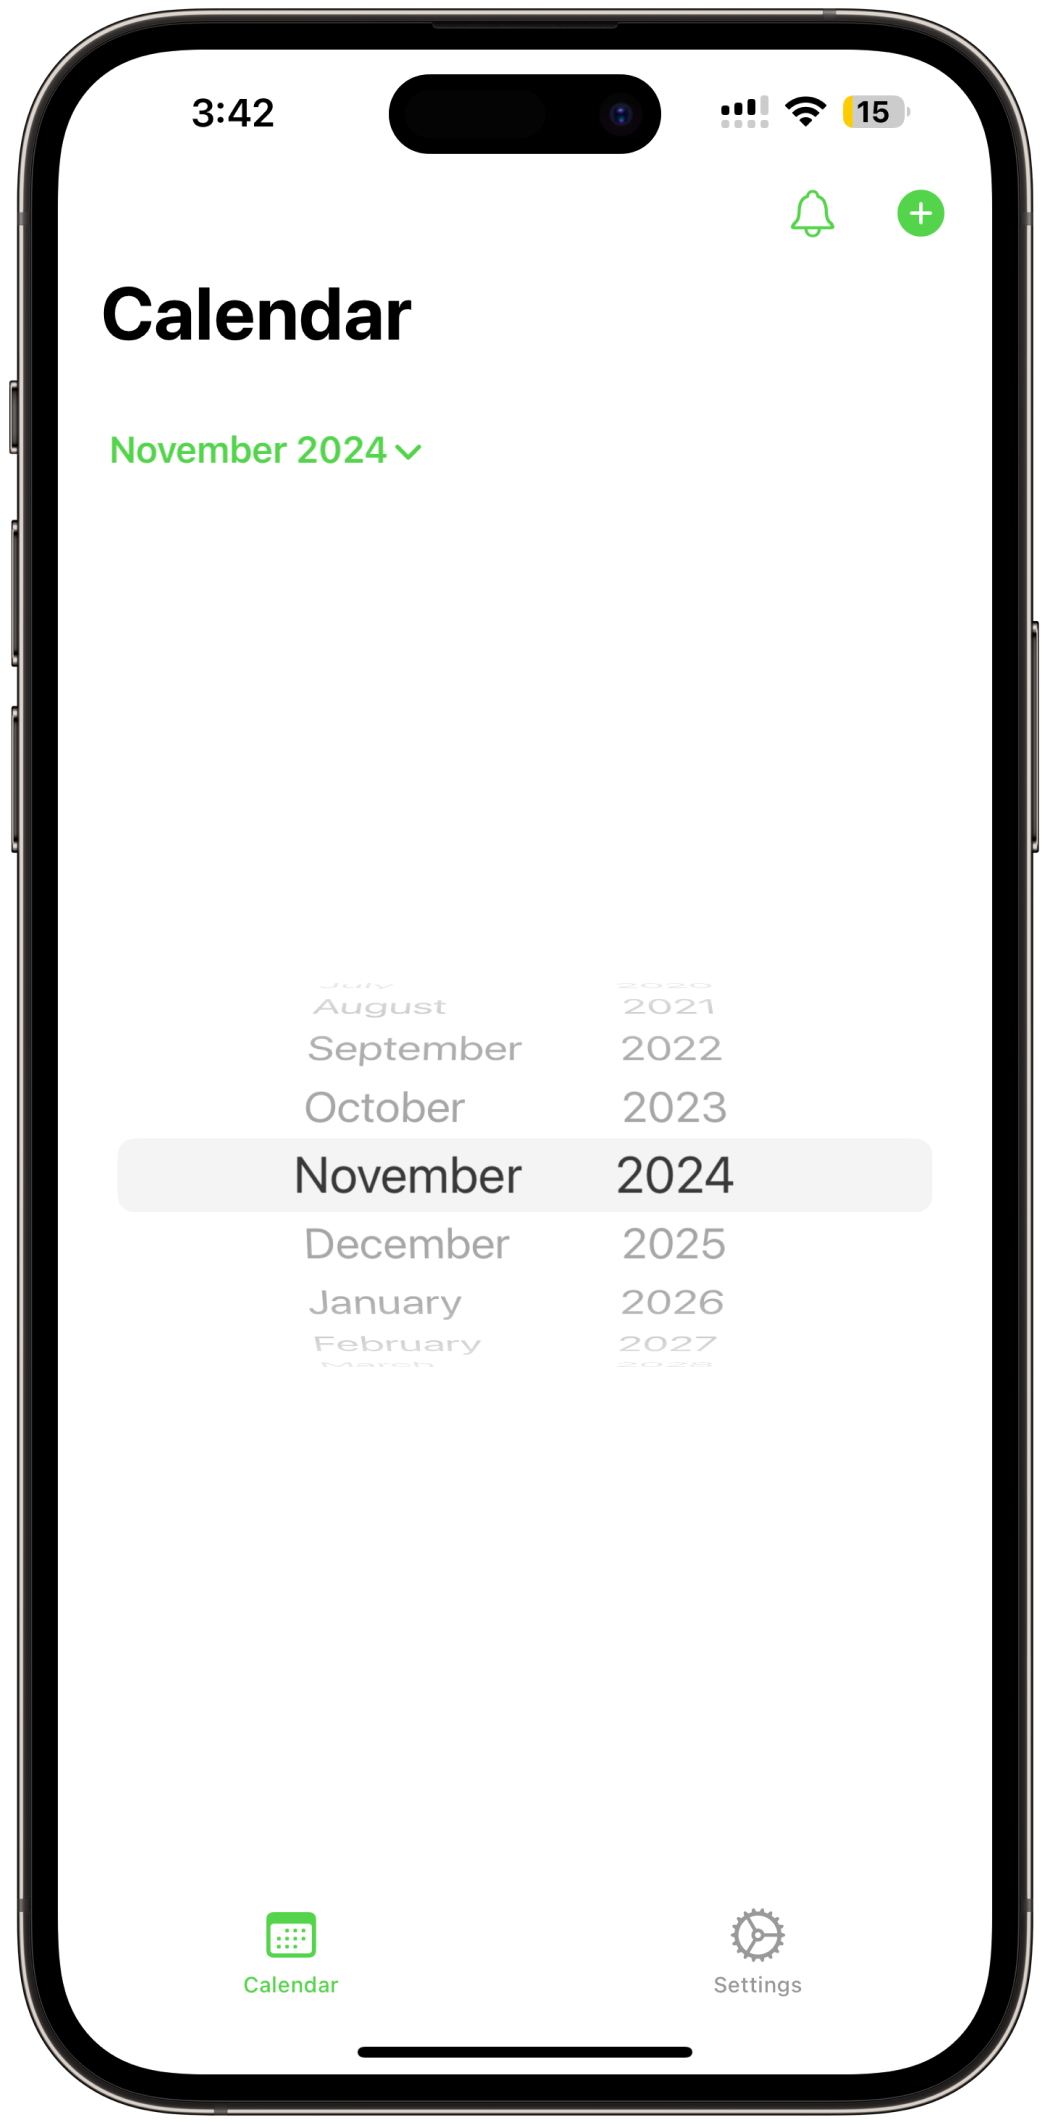
\includegraphics[width=\textwidth]{images/screen5.png}
        \caption{UI Screen 5: Add Event View - Time Selector}
        \label{fig:ui-screen-5}
    \end{minipage}
    \hfill
    \begin{minipage}{0.65\textwidth}
        Your explanation for Screen 3 goes here. This text will appear to the right 
        of the third screenshot. You can describe the final state of the interface 
        and what the user can accomplish on this screen.
    \end{minipage}
\end{figure}

\begin{figure}[!h]
    \begin{minipage}{0.65\textwidth}
        Your explanation for Screen 3 goes here. This text will appear to the right 
        of the third screenshot. You can describe the final state of the interface 
        and what the user can accomplish on this screen.
    \end{minipage}
    \hfill
    \begin{minipage}{0.3\textwidth}
        \centering
        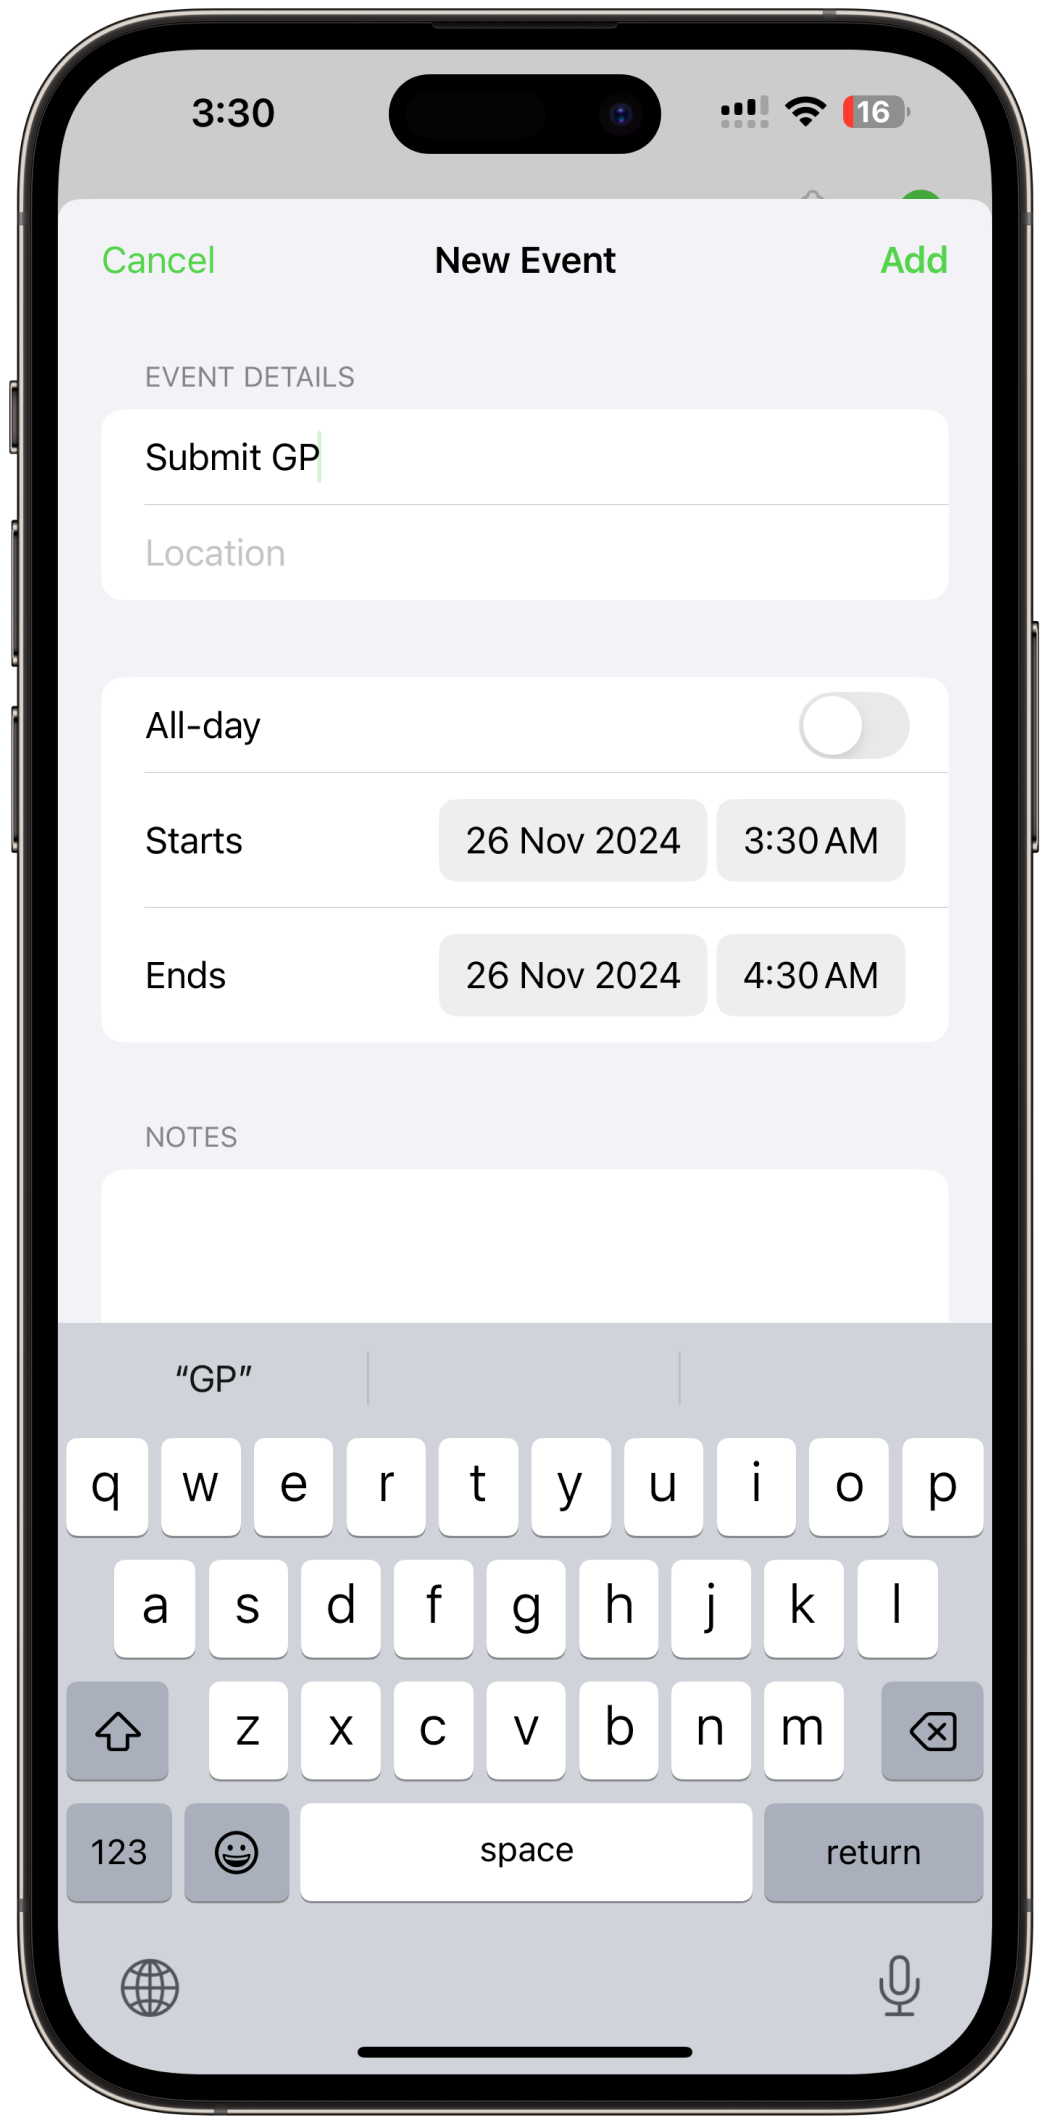
\includegraphics[width=\textwidth]{images/screen6.png}
        \caption{UI Screen 6: Add Event View - All-day}
        \label{fig:ui-screen-6}
    \end{minipage}
\end{figure}

\begin{figure}[!h]
    \begin{minipage}{0.3\textwidth}
        \centering
        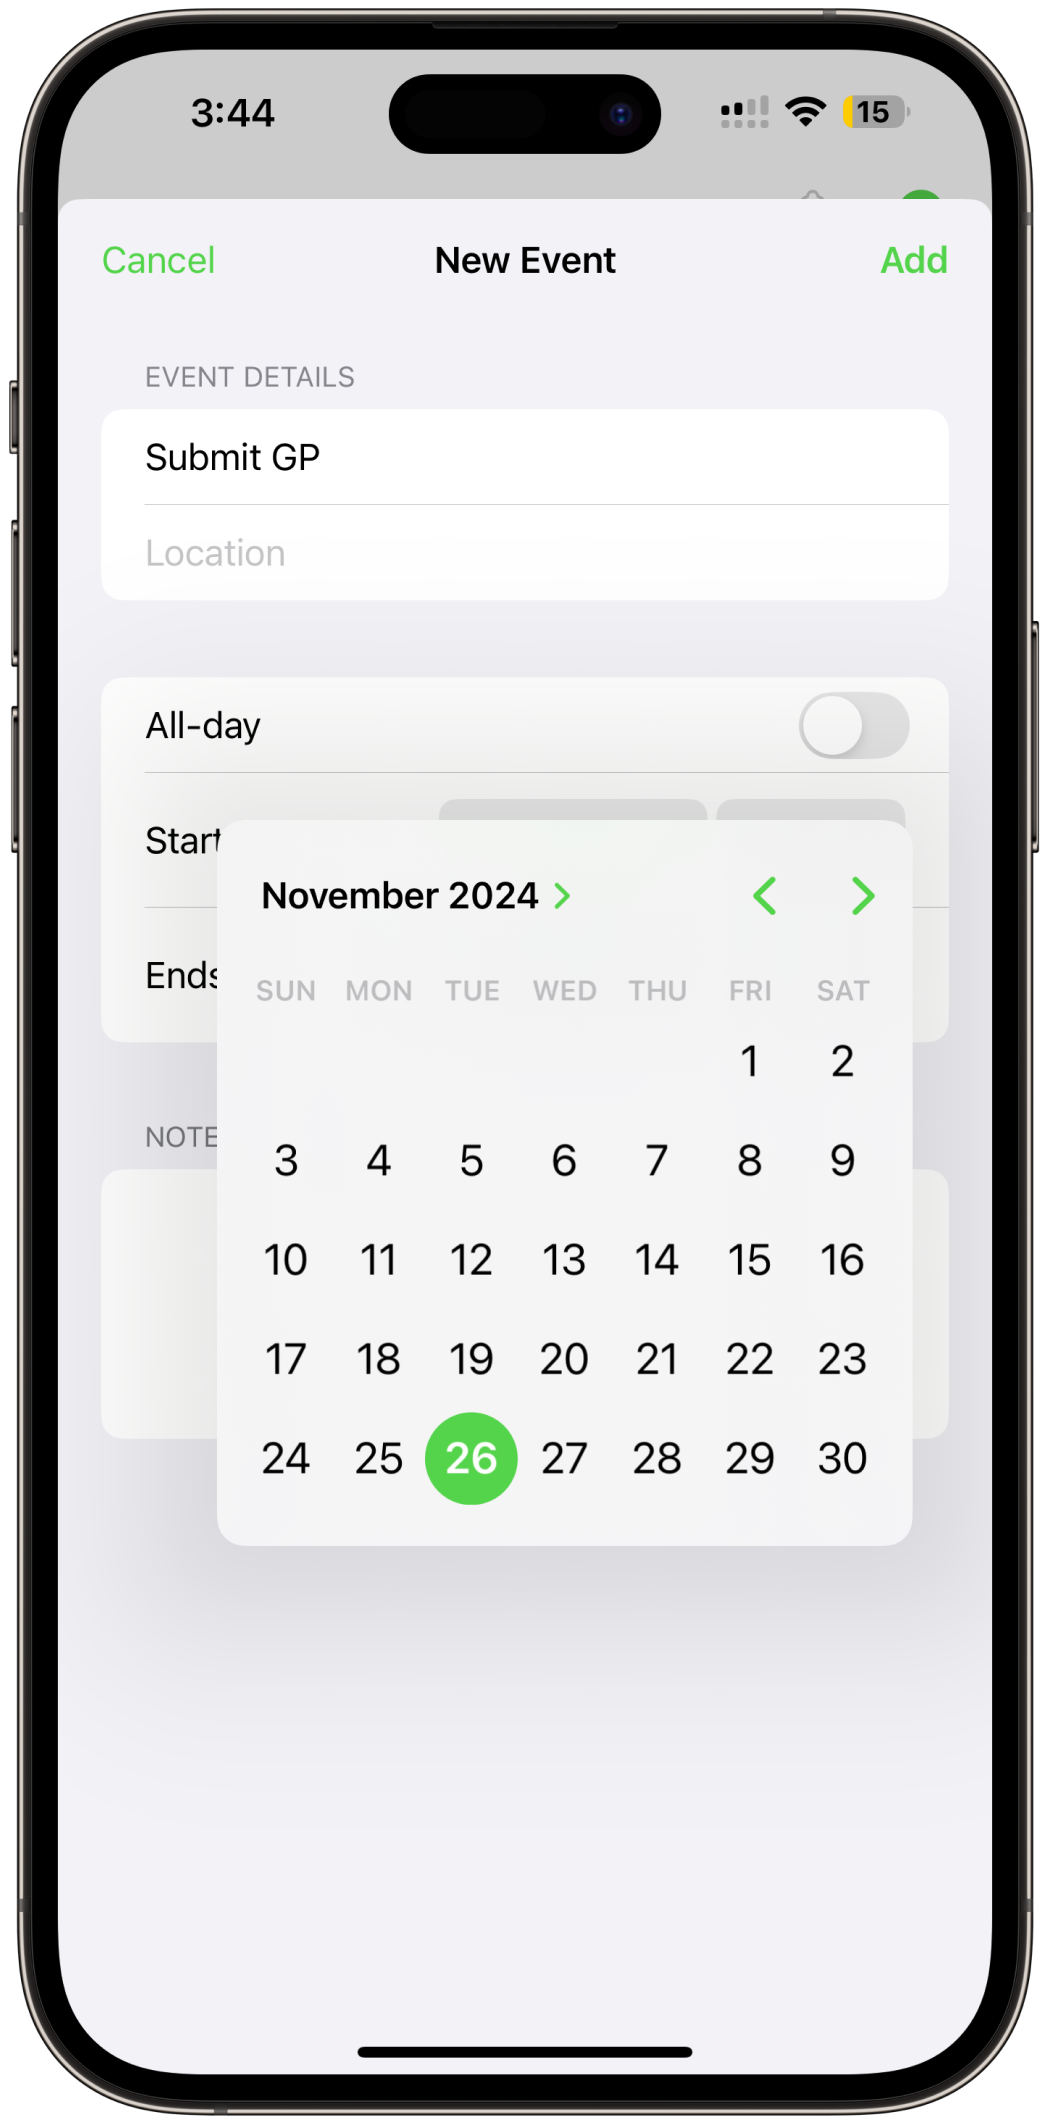
\includegraphics[width=\textwidth]{images/screen7.png}
        \caption{UI Screen 7: Settings View}
        \label{fig:ui-screen-7}
    \end{minipage}
    \hfill
    \begin{minipage}{0.65\textwidth}
        Your explanation for Screen 3 goes here. This text will appear to the right 
        of the third screenshot. You can describe the final state of the interface 
        and what the user can accomplish on this screen.
    \end{minipage}
\end{figure}